\documentclass[11pt]{article}
\usepackage{geometry}                % See geometry.pdf to learn the layout options. There are lots.
\geometry{letterpaper}                   % ... or a4paper or a5paper or ... 
%\geometry{landscape}                % Activate for for rotated page geometry
%\usepackage[parfill]{parskip}    % Activate to begin paragraphs with an empty line rather than an indent
\usepackage{graphicx}
\usepackage{amssymb}
\usepackage{amstext}
\usepackage{epstopdf}
\DeclareGraphicsRule{.tif}{png}{.png}{`convert #1 `dirname #1`/`basename #1 .tif`.png}

\title{Brief Article}
\author{The Author}
%\date{}                                           % Activate to display a given date or no date

\begin{document}
%\maketitle
\section{Some Power Considerations}

Let us think of a lineup as a head-to-head comparison of the data plot and $m-1$ null plots. Let the data plot have a $p$-value of $p_B$, and the null plots $p$-values of $p_{0, i}$ with $1 \le i \le m-1$.
We know that for each comparison the probability that the null plot has the smaller $p$-value is 
\begin{eqnarray*}
P(p_{i,0} < p_B) &=& \int_0^1  P(p_{i,0} \le p_B \mid p_B=t) f_{p_B}(t) dt =  \\
&=& \int_0^1 F_{p_{0,i}}(t) f_{p_B}(t) dt =  \int_0^1 t f_{p_B}(t) dt =  E[p_B],
\end{eqnarray*}
which, in particular, is independent of $p_{0,i}$ for all $i$.

Let us now define $X$ as the number of null plots in a lineup, for which the $p$-value $p_{0,i}$ is smaller than $p_B$ (i.e. under the assumption that the onlooker is able to identify the chart with the smallest $p$-value, they would pick any of the $X$  null plots over the data plot). 
Then $X \sim B_{m-1, E[p_B]}$, and the probability that an onlooker will pick the data plot in a given lineup is 
\begin{equation}\label{p0}
P(X=0) = \left(1 - E[p_B] \right)^{m-1} = P(p_B \le p_0),
\end{equation}
where $p_0 = \min_{1 \le i \le m-1}  \ p_{0,i}$

\section{Expected number of choices}
Since $X$ has a binomial distribution, we can have a look at the number of plots among the null plots that we would expect to be picked over the data plot:
\[
E[X] = (m-1)E[p_B].
\]
With an increase of the lineup size $m$ the number of null plots with a potentially stronger signal than the data plot grows linearly.
This allows us to infer some of the signal strength $p_B$ as
\[
E[p_B] = E[X]/(m-1),
\]
i.e. by averaging over the number of plots with  a stronger signal than the data plot we can evaluate signal strength of the plot even in the case where the data plot is not being picked by the observer:

assume that the same lineup plot is evaluated by $K$ independent observers. Wlog let the last plot be the data plot and plots 1 through $m-1$ the null plots. Let $n_i$ be the number of people who picked plot $i$ as the plot with the strongest expression of non-random structure, then $\sum_{k=1}^{m} n_k = K$, and $(n_1, n_2, ..., n_m) \sim$ Mult$_{\pi_1, ..., \pi_m}$ with $\sum_i \pi_i = 1$. We can estimate $\pi_i$ as $\widehat{\pi_i} = n_i/K$. 

We can then find an estimate for $X$, the number of null plots with a stronger signal than the data plot, as the number of null plots with more votes $n_i$ than the dataplot $n_m$. This gives an estimate for $X$ as
\[
\hat{X} = \sum_{i=0}^{m-1} I(n_i \ge n_m),
\]
where $I(x) = 1$ if $x$ is true and 0 otherwise.

However, this is not a very precise estimator for $E[p_B]$, since the only possible values for the  estimates are multiples of $1/(m-1)$.

As an alternative, we will make use of the fact that $\pi_m = P(X=0)$, since a vote for the dataplot implies that none of the other plots have a stronger signal.

With $\widehat{\pi_m} = n_m/K$ as an estimate for $\pi_m$, we get an plugin estimate for $E[p_B]$ from eq (\ref{p0}) as
\begin{equation}\label{signal}
\widehat{E[p_B]} = 1 - \left( \frac{n_m}{K} \right)^{1/(m-1)}.
\end{equation}

Since $n_m$ has a binomial distribution $n_m \sim B_{m-1, \pi_m}$, we can also derive a variance of the above estimate as
\[
Var \ \widehat{p_B} = K^{-2/(m-1)} Var \left[n_m^{1/(m-1)}\right]
\]

Figure \ref{fig:pval_plot_signal} shows a comparison of simulation based $p$-values resulting from model theory ($x$-axis) and graphical signal strength, defined in eq. (\ref{signal}) evaluated through experimentation.
Up to about a $p$-value of 0.15 there is a linear dependency between the two measures. Beyond that, the graphical signal strength flattens out. This `flattening out' is due to a reduction of the signal to noise ratio and is driven by the size $m$ of the lineup.
\begin{figure*}[hbtp]
   \centering
       \scalebox{0.6}{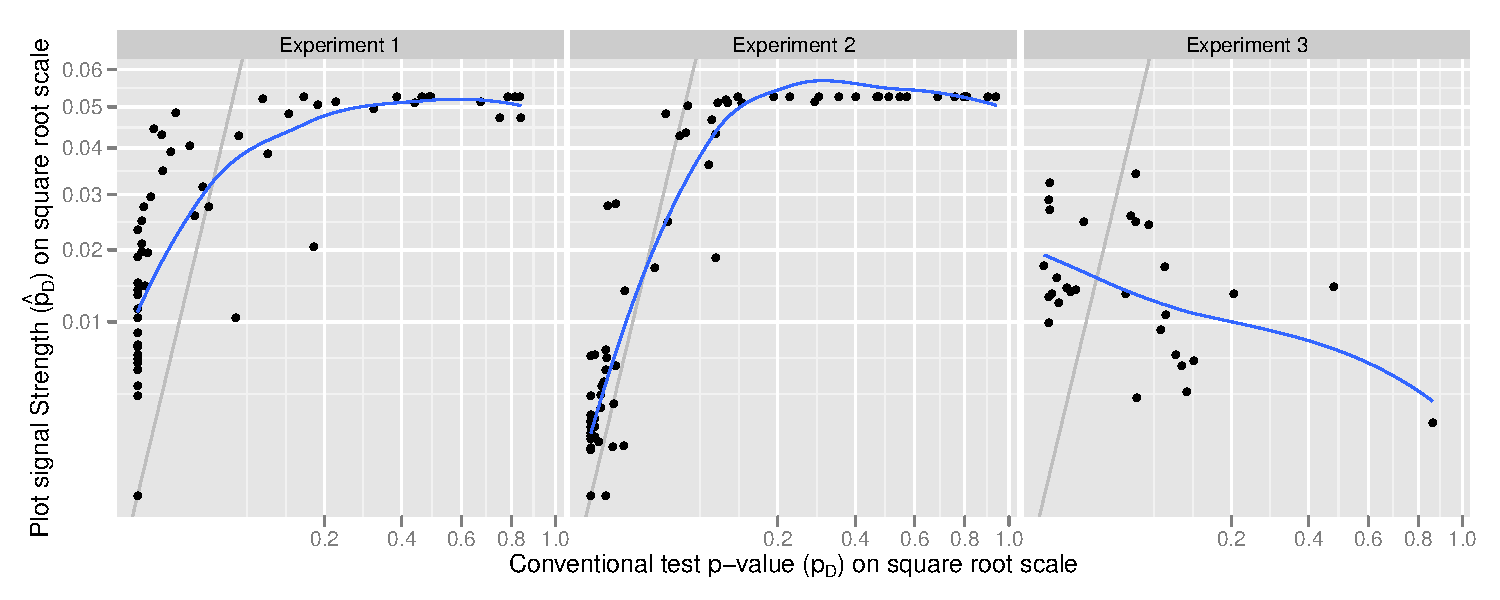
\includegraphics{images/p_val_plot_signal.pdf}}
       \caption{p-value vs plot signal strength. The solid line represents 45 degree line which represents the equity shown in equation (\ref{plot_signal}).}
       \label{fig:pval_plot_signal}
\end{figure*}



For the distribution of $n_m$, the number of times out of $K$ that observers picked the last plot to show the most non-random structure, we get
\[
n_m\sim \left \{ 
\begin{array}{cl}
B_{K, (1-E[p_B])^{m-1}} & \text { under } H_1\\
B_{K, 1/m} & \text { under } H_0
\end{array}
\right .
\]
Figure \ref{power} gives an overview of the probability of picking the dataplot for lineups of different size (as $m$ increases we have an increased probability to observe a more highly structured nullplot by chance).

\begin{figure}[htbp] %  figure placement: here, top, bottom, or page
   \centering
   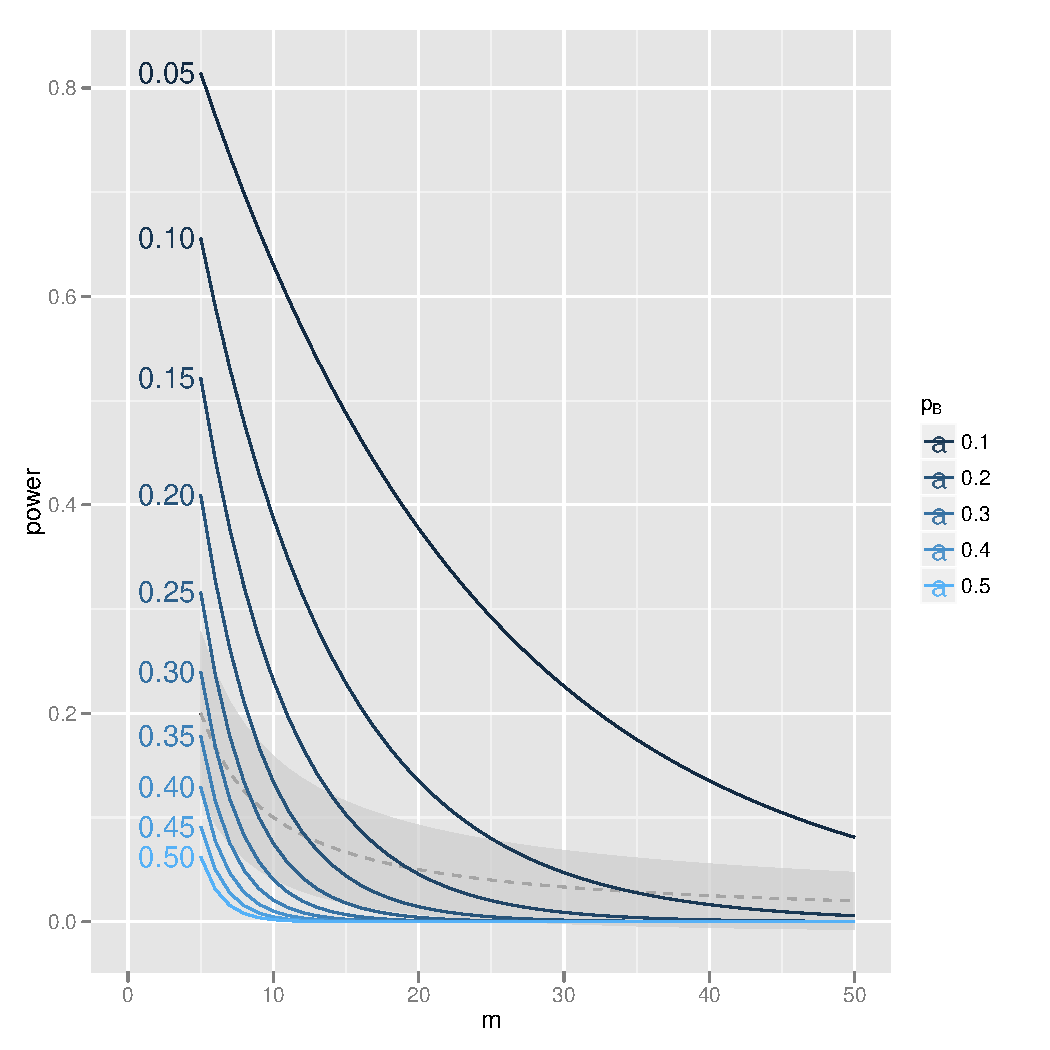
\includegraphics[width=2in]{images/powerplot.pdf} 
   \caption{Comparison of probabilities to pick the data plot for different size lineups $m$ and different values for data plot strength $p_B$. The grey line shows probability of picking the data plot under $H_0$. We see that for a $p$-value $p_B$ of about 0.15 for the dataplot the signal in the plot is so weak, that we cannot distinguish the dataplot from nullplots in a lineup of size $m=20$. }
   \label{power}
\end{figure}

\section{The Flattening out}
The flattening out in figure \ref{fig:pval_plot_signal} happens, when the signal in the data plot becomes too low to make it distinguishable from a nullplot. 
Under $H_0$ the $p$-value of the data plot $p_B \sim U[0,1]$. If we can assume that an observer is able to pick out the plot corresponding to the minimal $p$-value, we have a distribution of $Beta_{1, m}$ for the picked plot. 

\end{document}  